\chapter{The proposed centralized solution}\label{cha:existingSystem}

The \ref{PS:Q:Scalability} problem in the problem statement(\cref{sec:problemStatement}) requires a comparison on scalability in terms of numbers of turbines, between the decentralized solution and the current Siemens system. Ideally, for us to compare the two systems on equal terms, both systems should be implemented in the same environment. However, since we are only working with a small part of the current Siemens system, and do not have access to it or their test setup, we have chosen to build our own version of the current Siemens system, in the same environment as the decentralized solution.

This version of the current Siemens system, from now on referred to as the centralized solution, is built from what Siemens has informed about the current Siemens system. The goal of the centralized solution is to create a foundation for a comparison between the decentralized solution and the current Siemens system, by making the system architecture around the regulation algorithm the only difference between the centralized solution and the decentralized solution, thus ruling out the environment difference of the two systems as a parameter. The centralized solution is built to enable the collection of data that can be used to compare the two systems. We aim to compare the decentralized solution's test results with the centralized solution's test results, collected within the same environment, to accurately address the \cref{PS:Q:Scalability} problem.

In order to completely answer the \ref{PS:Q:Scalability} question, and compare the decentralized solution with the current Siemens system, another comparison must be introduced: A comparison between our centralized solution and the current Siemens system. This comparison is done in order to close the remaining 'comparison-gap' between the decentralized solution and the current Siemens system. 
This comparison will be based on information form Siemens and assumptions made when building the centralized solution.

There exist a difference between the current Siemens system and the centralized solution as well as a difference between the centralized solution and the decentralized solution, illustrated by deltas in \cref{fig:projectDiffOverview}.

\begin{figure}[!h]
	\centering
	\begin{tikzpicture}[
	node distance = 0.3cm,
	auto,
	block/.style={draw, rectangle, text width=5em, text centered, minimum height=5cm}		
	]
% Place nodes
\node [block]			(Siemens)												[label=above:Siemens system]	{};
\node []					(SimCen)		[right = of Siemens] 	{$\Delta$};
\node [block]			(OurCent)		[right = of SimCen] 	[label=above:Centralized solution]	{};

\begin{scope}[on background layer]
\node [block] 		(Central) 	[fit=(Siemens) (OurCent), inner sep=20pt] {};
\node []					(CenDece)		[right = of Central] 	{$\Delta$};
\node [block]			(DeCent)		[right = of CenDece] 	[label=above:Decentralized solution] {};
\end{scope}

\end{tikzpicture}
	\captionsetup{format=plain,font=footnotesize,labelfont={bf,defaultCapFont},labelsep=quad,singlelinecheck=no}
	\caption[Comparison overview]{
		\label{fig:projectDiffOverview} 
		\footnotesize{%
			Comparison overview.
		}
	}
\end{figure}

The delta between the current Siemens system and the centralized solution is minimized based on information delivered by Siemens Wind Power. Since the operation and regulation of the current Siemens system is proprietary the full system information is not available. To make up for the missing information a number of assumptions has been made about the current Siemens system which is also a part of the delta.

The thesis motivation (\cref{sec:ThesisMotivation}) describes a brief overview of the current Siemens system. This chapter gives a description of the regulation algorithm, which is a key component of the current Siemens system. Furthermore the chapter describes the centralized solution followed by a theoretical comparison between the centralized solution and the current Siemens system. 

\section{Regulation algorithm}\label{sec:cenRegAlgorithm}
The regulation algorithm is a key component of the current Siemens system and it is where new setpoints are calculated. Since it is not the purpose of this thesis to improve the regulation algorithms, the regulation algorithm has been considered a black box in the development of both the centralized and the decentralized solution. What is important to this thesis is that the algorithm used is the same in both the centralized and the decentralized solution, to make sure the two solutions are compared on the same terms. 

%To get as realistic a picture of the system as possible of the regulation algorithm, we tried to gain access to the algorithm Siemens currently use, but due to the regulation algorithm at Siemens being a commercial secret, this was not possible.

\begin{figure}
	\centering
	\begin{tikzpicture}[
	point/.style={inner sep=0pt}, %circle,minimum size=2pt,fill=red},
	textNode/.style={inner sep=2pt},
	hv path/.style={to path={-| (\tikztotarget)}},
	vh path/.style={to path={|- (\tikztotarget)}},
	skip loop h/.style={to path={-- ++(0,#1) -| (\tikztotarget)}},
	skip loop v/.style={to path={-- ++(#1,0) |- (\tikztotarget)}},
	graphs/every graph/.style={edges=rounded corners}
	]
	
% Place nodes
\matrix[row sep=1.4cm,column sep=.4cm] {
	\node [point]  		(p1x1)	{}; &&
	\node [rectangle]	(Turbine)		[draw, label=above:\textbf{$\cdot$}N Turbines, text width=50pt]	{Cur.Prod. Max.Prod}; &&
	\node [point]  		(p1x3)	{}; \\
	
	\node [point]  		(p2x1)			{}; &&
	\node [textNode]	(HPPP)		 	{Reg. algorithm}; &&
	\node [textNode]	(Setpoint)	{N Setpoints}; \\

	&& \node [textNode]  (gSetpoint)							{Global SetPoint}; \\
};
	
\graph[use existing nodes]{
	Turbine ->[skip loop v=-3.1cm] HPPP -> Setpoint ->[vh path] Turbine;
	gSetpoint -> HPPP;
};

\end{tikzpicture}



%\begin{tikzpicture}[
%	point/.style={inner sep=0pt}, %circle,minimum size=2pt,fill=red},
%	textNode/.style={inner sep=2pt},
%	hv path/.style={to path={-| (\tikztotarget)}},
%	vh path/.style={to path={|- (\tikztotarget)}},
%	skip loop h/.style={to path={-- ++(0,#1) -| (\tikztotarget)}},
%	skip loop v/.style={to path={-- ++(#1,0) |- (\tikztotarget)}},
%	graphs/every graph/.style={edges=rounded corners}
%	]
%	
%% Place nodes
%\matrix[row sep=1.5cm,column sep=.5cm] {
%	\node [point]  		(p1x1)	{}; &&
%	\node [rectangle]	(Turbine)		[draw, label=above:\textbf{$\cdot$}N Turbines, text width=50pt]	{Cur.Prod. Max.Prod}; &&
%	\node [point]  		(p1x3)	{}; \\
%	
%	\node [point]  		(p2x1)			{}; &&
%	\node [textNode]	(HPPP)		 	{HPPP}; &&
%	\node [textNode]	(Setpoint)	{\textbf{$\cdot$}N Setpoints}; \\
%
%	\node [textNode]  (gSetpoint)										{Global SetPoint}; &&
%	\node [rectangle]	(Data)			[draw, text width=50pt] {Cur.prod  Max.Prod};\\
%};
%
%\node [textNode,right of=Data] {~~~~~~~~~~~~~~~~~\textbf{$\cdot$}N Turbines};
%	
%\graph[use existing nodes]{
%	Turbine ->[skip loop v=-2.7cm] HPPP -> Setpoint ->[vh path] Turbine;
%	gSetpoint.east -> HPPP;
%	Data -> HPPP;
%};
%
%\end{tikzpicture}

	\captionsetup{format=plain,font=footnotesize,labelfont={bf,defaultCapFont},labelsep=quad,singlelinecheck=no}
	\caption[Centralized input/output parameters of the regulation algorithm]{
		\label{fig:ioCenRegAlg} 
		\footnotesize{%
			Centralized input/output parameters of the regulation algorithm.
		}
	}
\end{figure}

With the algorithm being a black box, the input/output parameters where studied to provide the optimal network communication around the regulation algorithm. \Cref{fig:ioCenRegAlg} presents a simple input/output overview of the regulation algorithm. The Input/output parameters are as follows:

\begin{description}
	\item The \textbf{global setpoint} of the wind farm. This is the production production setpoint for the entire wind farm. %Which means all turbines combined should produce.
	\item The \textbf{setpoint} of each turbine, calculated from the regulation algorithm. 
	\item The \textbf{current production} of the turbine.
	\item The \textbf{maximum production} of the turbine. The data is provided by Siemens, this parameter is primarily determined from the wind conditions around the turbine.
\end{description}

These input/output parameters of the regulation algorithm are simplified compared to the current Siemens system and only regulates active power production. The data used is more og less irrelevant for the purpose of this thesis as long as both the decentralized solution and the centralized solution are using the same data and as long as both systems are able to perform the same simple regulation.
The data used is for adding dynamic to the setup and does not impact regulation performance.

\section{Regulation cycle}\label{sec:currentSystemCen} 

The first area studied when building the centralized solution, was building the frames for the regulation algorithm, meaning how to communicate the input/output parameters between Park Pilot and turbines in the centralized solution.

This section describes the components of a regulation cycle in the centralized solution. The regulation cycle consist of a number of steps presented in \cref{fig:timingCentral}.

\begin{figure}[!h]
	%The figure show how regulation time differs central vs decantral
	

{ %The brackets issolate the enviroment

\tikzstyle{line}		 	= [draw]

\makeatletter
\ifcsname c@wavenum\endcsname %Only create one counter
\else
	\newcounter{wavenum}
\fi
\makeatother

\newcommand*{\bitvector}[3]{
  \draw[fill=#3] (t_cur) -- ++( .1, .3) -- ++(#2-.2,0) -- ++(.1, -.3)
                         -- ++(-.1,-.3) -- ++(.2-#2,0) -- cycle;
  \path (t_cur) -- node[anchor=mid](textNode) {#1} ++(#2,0) node[time] (t_cur) {};
  }

% \known{val}{length}
\newcommand*{\known}[2]{
    \bitvector{#1}{#2}{white}
}

% \unknown{length}
\newcommand*{\unknown}[2]{
    \bitvector{#1}{#2}{black!20}
}

% \nextwave{name}
\newcommand{\nextwave}[1]{
  %\path (0,\value{wavenum}) node[time] (t_cur) {};
   \path (0,\value{wavenum}) node[left] {#1} node[time] (t_cur) {};
  \addtocounter{wavenum}{-1}
}

\newcommand{\timeSpanLabel}{
	\node (CycleTimeLabel) [rectangle, above = 0.7cm of textNode, inner sep=0pt] {Regulation cycle time};	  
}

\newcommand{\timeSpanA}{
	\node (t_timeSpanA) [point, above = 0 of t_cur] {};	  
}

\newcommand{\timeSpanB}{
	\node (t_timeSpanB) [point, above =0 of t_cur] {};

  \graph[use existing nodes]{
  	t_timeSpanA --[time span=1cm] CycleTimeLabel;
   	CycleTimeLabel.south --[time span=-0.24cm] t_timeSpanB;
  }; 
    	
}


%%% End of timing.sty
\begin{tikzpicture}[
	point/.style={inner sep=0pt}, %circle,minimum size=2pt,fill=red},
	draw=black, 
	yscale=.8,
	xscale=1,
	hv path/.style={to path={-| (\tikztotarget)}},
	vh path/.style={to path={|- (\tikztotarget)}},
	skip loop v/.style={to path={-- ++(#1,0) |- (\tikztotarget)}},		
	skip loop h/.style={to path={-- ++(0,#1) -| (\tikztotarget)}},
	time span/.style={to path={-- ++(0,#1) -| (\tikztotarget)}},
	graphs/every graph/.style={edges=rounded corners}	
	]
	
  \tikzstyle{time}=[coordinate]
  \setlength{\unitlength}{1cm}
  \setcounter{wavenum}{0}
    
  %\nextwave{Regulation Time} \unknown{SendData}{2} \known{WaitForData}{5} \unknown{ReciveData}{2} \unknown{Calculate}{2}\unknown{SendSP}{2}
  \nextwave{Park Pilot} \unknown{reqStates}{1.8} \known{wait}{2} \unknown{readStates}{2} \unknown{regAlg.}{1.7} \unknown{sendSetpoints}{2.6}
  
  \nextwave{Turbine} \known{wait}{1.8} \unknown{replyState}{2} \known{wait}{6.3} \unknown{receiveSetpoint}{2.9}
    
  
\end{tikzpicture}
}

	\caption{The regulation cycle of the centralized solution}
	\label{fig:timingCentral}
\end{figure}

\subsection{Get turbine states}\label{sec:getTurbineStates}

\begin{figure}
	\centering
	\begin{sequencediagram} %Created using pgf-umlsd
		\newthread{parkPilot}{:Park Pilot}
		\newthread{turbineDataReplier}{:Turbine Data Replier}
		\newinst{turbine}{:Turbine}
	
		\begin{sdblock}{each turbine}{}
			\mess[1]{parkPilot}{reqState}{turbineDataReplier}
			\begin {call}{turbineDataReplier}{readState()}{turbine}{return state}
			\end {call}
			\mess[1]{turbineDataReplier}{replyState}{parkPilot}
		\end{sdblock}				
	\end{sequencediagram}

	\captionsetup{format=plain,font=footnotesize,labelfont={bf,defaultCapFont},labelsep=quad,singlelinecheck=no}
	\caption[First part of the regulation cycle]{
		\label{fig:getStatesOfTurbines} 
		\footnotesize{%
			First part of the regulation cycle: Getting the state of all turbines.
			\todo[inline]{Hvilken bedre forståelse får man ved at have mellem ledet på?}
		}
	}
\end{figure}
In order for the Park Pilot to calculate turbine setpoints, the Park Pilot must have the state of all turbines.
A simple overview of the first part of the regulation cycle is presented in \cref{fig:getStatesOfTurbines}. This part of the regulation cycle is implemented using the RTI Connext Request-Reply API~\cite{rtiConnextUsersManual}. The three primary objects associated with retrieving states are:

\begin{description}
	\item [Park Pilot] The Park Pilot requests the current state from all turbines and calculates setpoints when states has been received.
	\item [Turbine Data Replier] The replier object handles the request messages and sends state data in the reply messages.
	\item [Turbine] The underlying turbine object is the interface to the Turbine, which handles communication with the underlying database with simulation data.
\end{description}

The Park Pilot sends a request to a specific DDS Topic and then waits until it has received a reply from all the turbines subscribing to this DDS Topic, which in our case is all turbines. In a real-life implementation of the centralized solution, a timer should be implemented to determine how long to wait for the replies. The turbine should be marked as offline, if it does not reply within that time frame. However, since this is a prototype for comparison purposes only, this functionality has not been implemented. The request message sent from the Park Pilot contains the regulation cycle time, which is only used for data logging purposes.

The Turbine Data Replier is associated with a Turbine object and runs on every turbine. After instantiation the Turbine Data Replier starts an infinite loop which first waits until a request is received, reads turbine data from the Turbine object and finally sends a reply containing the data to the Park Pilot. 
%Ideally, the Turbine Data Replier object should have been implemented as a listener on the request topic using RTI Connext SimpleReplier~\cite{rtiConnextUsersManual}. However, we could not get it to work using the SimpleReplier but waiting infinitely for a request works just as well for our purpose.

The Turbine object is the interface to the Turbine simulator. The primary functionality of this object is to change state when a new setpoint is assigned to the object. Furthermore it reads data from the underlying MongoDB database. 

\subsection{Calculate setpoints (regAlgorithm)}\label{sec:calculateSetpoints}

When the Park Pilot has received the states of all turbines the setpoints for all turbines are calculated. Since we don't have access to Siemens' regulation algorithm (see \cref{sec:cenRegAlgorithm} for explanation), we have developed our own simple regulation algorithm. The code for this regulation algorithm is presented in \cref{fig:cenRegAlgCode}.

\begin{figure}[!h]
	\centering
%	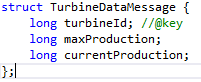
\includegraphics[width=0.3\textwidth,natwidth=250,natheight=200]{turbineDataMessage.PNG} 
	\begin{lstlisting}[language=C++,tabsize=2,basicstyle=\small]
void CentralizedParkPilot::regAlgorithm(
	uint_fast32_t globalSetpoint,
	LoanedSamples<TurbineDataMessage> &turbines)
{
	int availableTurbinesCount = turbines.length();

	typedef LoanedSamples<TurbineDataMessage>::iterator iterator;
	long localSetpoint = 0;

	for (iterator it = turbines.begin(); it != turbines.end(); ++it) {
		if (it->info().valid_data) {

			if (it->data().currentProduction >= it->data().maxProduction) {
				availableTurbinesCount--;
			}
		}
		else
			availableTurbinesCount--;
	}

	for (iterator it = turbines.begin(); it != turbines.end(); ++it) {
		if (it->info().valid_data) {
			if (availableTurbinesCount <= 0)
				localSetpoint = globalSetpoint;
			else
				localSetpoint = globalSetpoint / availableTurbinesCount;

			if (localSetpoint > it->data().maxProduction) {
				localSetpoint = it->data().maxProduction;
			}

			_turbineOutlets[it->data().turbineId - START_ID]->
						setSetpoint(localSetpoint);
					
			_turbineOutlets[it->data().turbineId - START_ID]->publishData();
		}
	}
}
	\end{lstlisting}
	\captionsetup{format=plain,font=footnotesize,labelfont={bf,defaultCapFont},labelsep=quad,singlelinecheck=no}
	\caption[The regulation algorithm of the centralized solution]{
		\label{fig:cenRegAlgCode} 
		\footnotesize{%
			Code for the centralized regulation algorithm used to calculate setpoints.
			\todo[inline]{Høre det ikke til i et appendix? Måske kan det omskrives til mere kompakt psedu kode og stadigvæk bruges.}
		}
	}
\end{figure}


Our regulation algorithm works by first determining how many turbines that are available for production. This is done going through every turbine, checking if they currently hit their maximum production capacity. If a given turbine is producing at maximum capacity, a greater load cannot be assigned to it and the available turbine count is reduced. 

Next the setpoint for every turbine is calculated using this simple formula: $setpoint=globalSetpoint/availableTurbines$. If this new setpoint is higher than the maximum capacity of a given turbine, the turbine is set to produce at maximum capacity. If this happens, a gap between the maximum capacity and the calculated setpoint is left unhandled, and the wind farm is under-producing until the next cycle, where a new set of setpoints are calculated, with one less available turbine. Hence this gap will eventually be closed unless the maximum capacity of the entire park is reached.

\subsection{Send setpoints}

\Cref{fig:sendSetpoints} presents a simple overview of the last part of the regulation cycle. This part of the regulation cycle is implemented using RTI Connext Publish-Subscribe API~\cite{rtiConnextUsersManual}. The primary objects are:

\begin{description}
	\item [Park Pilot] Explained in \cref{sec:getTurbineStates}.
	\item [Turbine Outlet] The Park Pilots implementation of a given turbine. One Turbine Outlet is instantiated on the Park Pilot for each turbine in the park. Writing data to each turbine is handled from this object.
	\item [Setpoint Listener] The listener object called when when a new setpoint is published. One Setpoint Listener are instantiated on each turbine.
	\item [Turbine] Explained in \cref{sec:getTurbineStates}.
\end{description}

After calculating the setpoints (\cref{sec:calculateSetpoints}), the Park Pilot sends a new setpoint to each turbine. The Park Pilot sets the setpoint of the Turbine Outlet before publishing the Data.

\begin{figure}[!h]
	\centering
	\begin{sequencediagram} %Created using pgf-umlsd
		\newthread{parkPilot}{:Park Pilot}
		\newinst{turbineOutlet}{:Turbine Outlet}
		\newinst{setPointListener}{:Setpoint Listener}
		\newinst{turbine}{:Turbine}
	
		\begin{sdblock}{each turbineOutlet}{}
			\begin {call}{parkPilot}{setSetpoint()}{turbineOutlet}{}
			\end {call}
			\begin {call}{parkPilot}{publishData()}{turbineOutlet}{}
				\mess[1]{turbineOutlet}{write}{setPointListener}
				\begin {call}{setPointListener}{setSetpoint()}{turbine}{}
				\end {call}
			\end {call}
		\end{sdblock}				
	\end{sequencediagram}

	\captionsetup{format=plain,font=footnotesize,labelfont={bf,defaultCapFont},labelsep=quad,singlelinecheck=no}
	\caption[Last part of the regulation cycle]{
		\label{fig:sendSetpoints} 
		\footnotesize{%
			Last part of the regulation sequence: Sending setpoints to all turbines.
		}
	}
\end{figure}

The main purpose of Turbine Outlet object is to register and publish setpoints to each turbine. Upon instantiation, the Turbine Outlet registers the turbine id as a RTI Connext key~\cite{rtiConnextUsersManual} to the setpoint topic and saves the handle object. Saving the handle upon registration and using the handle when writing improves performance~\cite{DDSInstanceHandlet}, which is why the handle is saved with the object. Lastly the object writes the data to the topic.
\todo[inline]{Does the metioning of the handle object bring anything new to the reader except for confusion of a new tearm? To my knowledge handle object only help preallocate and therefore only improve performance during startup which we dont messure...}

The Setpoint Listener object listens on a Content Filtered Topic~\cite{rtiConnextUsersManual}, the listener only reacts to messages with a key that equals the turbines id. When Setpoint Listener object is invoked, the new setpoint is saved to the Turbine object, which updates the state of the turbine.

\section{DDS configuration}\label{sec:ddsConfigCen} 

The key component used for communication is DDS (see \cref{sec:DSM})\todo{Hvorfor refferes der til Distributed shared memory?}. This section describes how DDS has been configured for the centralized solution.

\subsection{Interface Definition Language}\label{sec:cenIdl}

The data transfer objects (DTO) used when sending messages from the turbines to the Park Pilot, and the other way around, are created using the RTI Connext Interface Definition Language~\cite{rtiConnextUsersManual}. DTOs are defined in an IDL file. From there the actual implementations of the IDL definitions are auto generated from the command prompt using the \textit{rtiddsgen}~\cite{rtiConnextUsersManual} command.

\begin{figure}[!h]
	\centering
%	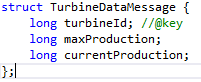
\includegraphics[width=0.3\textwidth,natwidth=250,natheight=200]{turbineDataMessage.PNG} 
	\begin{lstlisting}[language=C++,tabsize=2,basicstyle=\small]
	struct TurbineDataMessage {
		long turbineId; //@key
		long maxProduction;
		long currentProduction;	
	}	
	\end{lstlisting}
	\captionsetup{format=plain,font=footnotesize,labelfont={bf,defaultCapFont},labelsep=quad,singlelinecheck=no}
	\caption[Centralized turbine reply message]{
		\label{fig:cenTurbineDataMessage} 
		\footnotesize{%
			The reply message .idl file sent from the turbines to the Park Pilot in the centralized solution.
		}
	}
\end{figure}

\begin{figure}[!h]
	\centering
	%	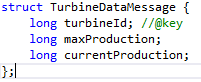
\includegraphics[width=0.3\textwidth,natwidth=250,natheight=200]{turbineDataMessage.PNG} 
	\begin{lstlisting}[language=C++,tabsize=2,basicstyle=\small]
	struct SetpointMessage {
		long turbineId; //@key
		long setPoint;
	};	
	\end{lstlisting}
	\captionsetup{format=plain,font=footnotesize,labelfont={bf,defaultCapFont},labelsep=quad,singlelinecheck=no}
	\caption[Centralized Park Pilot setpoint message]{
		\label{fig:cenTurbineSetpointMessage} 
		\footnotesize{%
			The setpoint message .idl file sent from the the Park Pilot to the turbines in the centralized solution.
		}
	}
\end{figure}

\begin{figure}[!h]
	\centering
	%	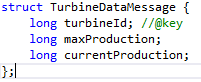
\includegraphics[width=0.3\textwidth,natwidth=250,natheight=200]{turbineDataMessage.PNG} 
	\begin{lstlisting}[language=C++,tabsize=2,basicstyle=\small]
	struct RequestMessage {
		long msSinceLastWrite;
	};	
	\end{lstlisting}
	\captionsetup{format=plain,font=footnotesize,labelfont={bf,defaultCapFont},labelsep=quad,singlelinecheck=no}
	\caption[Centralized Park Pilot request message]{
		\label{fig:cenTurbineRequestMessage} 
		\footnotesize{%
			The request message .idl file sent from the Park Pilot to the turbines in the centralized solution.
		}
	}
\end{figure}

The IDL definitions are defined by observing what data to transfer between the turbines and the Park Pilot. As an example \cref{fig:cenTurbineDataMessage} is the IDL definition of the data transfer object used to reply state from the turbines to the Park Pilot.

%\subsection{Topics}
%
%Including the topics generated from the RTI Connext Request-Reply implementation~\cite{rtiConnextUsersManual} the following topics are used:
%
%\begin{figure}
%	\centering
%	\begin{tikzpicture}[
	point/.style={inner sep=0pt}, %circle,minimum size=2pt,fill=red},
	textNode/.style={inner sep=2pt},
	hv path/.style={to path={-| (\tikztotarget)}},
	vh path/.style={to path={|- (\tikztotarget)}},
	skip loop h/.style={to path={-- ++(0,#1) -| (\tikztotarget)}},
	skip loop v/.style={to path={-- ++(#1,0) |- (\tikztotarget)}},
	graphs/every graph/.style={edges=rounded corners}
	]
	
% Place nodes
\matrix[row sep=1.4cm,column sep=.4cm] {
	\node [point]  		(p1x1)	{}; &&
	\node [rectangle]	(Turbine)		[draw, label=above:\textbf{$\cdot$}N Turbines, text width=50pt]	{Cur.Prod. Max.Prod}; &&
	\node [point]  		(p1x3)	{}; \\
	
	\node [point]  		(p2x1)			{}; &&
	\node [textNode]	(HPPP)		 	{Reg. algorithm}; &&
	\node [textNode]	(Setpoint)	{N Setpoints}; \\

	&& \node [textNode]  (gSetpoint)							{Global SetPoint}; \\
};
	
\graph[use existing nodes]{
	Turbine ->[skip loop v=-3.1cm] HPPP -> Setpoint ->[vh path] Turbine;
	gSetpoint -> HPPP;
};

\end{tikzpicture}



%\begin{tikzpicture}[
%	point/.style={inner sep=0pt}, %circle,minimum size=2pt,fill=red},
%	textNode/.style={inner sep=2pt},
%	hv path/.style={to path={-| (\tikztotarget)}},
%	vh path/.style={to path={|- (\tikztotarget)}},
%	skip loop h/.style={to path={-- ++(0,#1) -| (\tikztotarget)}},
%	skip loop v/.style={to path={-- ++(#1,0) |- (\tikztotarget)}},
%	graphs/every graph/.style={edges=rounded corners}
%	]
%	
%% Place nodes
%\matrix[row sep=1.5cm,column sep=.5cm] {
%	\node [point]  		(p1x1)	{}; &&
%	\node [rectangle]	(Turbine)		[draw, label=above:\textbf{$\cdot$}N Turbines, text width=50pt]	{Cur.Prod. Max.Prod}; &&
%	\node [point]  		(p1x3)	{}; \\
%	
%	\node [point]  		(p2x1)			{}; &&
%	\node [textNode]	(HPPP)		 	{HPPP}; &&
%	\node [textNode]	(Setpoint)	{\textbf{$\cdot$}N Setpoints}; \\
%
%	\node [textNode]  (gSetpoint)										{Global SetPoint}; &&
%	\node [rectangle]	(Data)			[draw, text width=50pt] {Cur.prod  Max.Prod};\\
%};
%
%\node [textNode,right of=Data] {~~~~~~~~~~~~~~~~~\textbf{$\cdot$}N Turbines};
%	
%\graph[use existing nodes]{
%	Turbine ->[skip loop v=-2.7cm] HPPP -> Setpoint ->[vh path] Turbine;
%	gSetpoint.east -> HPPP;
%	Data -> HPPP;
%};
%
%\end{tikzpicture}
%
%	\captionsetup{format=plain,font=footnotesize,labelfont={bf,defaultCapFont},labelsep=quad,singlelinecheck=no}
%	\caption[Regulation aslgorithm input/output parameters]{
%		\label{fig:ioRegAlg} 
%		\footnotesize{%
%			Input/output parameters of the regulation algorithm.
%		}
%	}
%\end{figure}

\subsection{Choosing quality of service parameters}\label{sec:choosingQosParams}

Quality of Service (QoS) parameters are parameters used to determine the behavior of a system using RTI Connext DDS. As such, setting the right QoS parameters for the centralized solution is important in order to duplicate the behavior of the current Siemens system as closely as possible. 

In order to decide the QoS parameters for the centralized solution, the QoS XML file from the current system at Siemens was provided by Siemens and can be found in \cref{appendix:siemensQosFile}. Thus QoS parameters for the centralized solution has been set using this file, which presents many different QoS profiles.

The Siemens QoS XML file specifies one DomainParticipantFactory profile. This profile has been applied to the solution and parameters irrelevant to the purpose of this thesis has been removed from the profile.\todo[inline]{Gives very little to no information, explain what has been removed or delete?}

The Siemens QoS XML file specifies two DomainParticipant profiles. One using UDPv4 and one using DTLS as transport plugin. The one using UDPv4 has been chosen for the centralized solution, since DTLS encryption and decryption is an unnecessary overhead, that either should be used for both the centralized- and the decentralized solution or for neither, in order for the two solutions to be compared on equal terms. Thus for simplicity neither of the solutions use DTLS.

As for DataReaders, DataWriters and Topics, the file specifies multiple profiles the use of which is unknown. Thus it is unknown which ones has been used for the part of the system that is implemented with the centralized solution. Furthermore since the centralized solution is a simplified version of the current Siemens system it will not need the number of DataReaders, DataWriters and Topics that the current Siemens system apply.
\todo[inline]{The difference should be explained, we need to argue the use better...}

Each QoS parameter in every QoS profile has been evaluated and the parameters relevant to the purpose of this theses has been applied to the centralized solution, based on assumptions about the current Siemens system. The QoS XML file roughly presents profiles that combines the following parameters in different ways:

\paragraph{Reliability} is the QoS parameter, which determines whether or not data published by a DataWriter will be reliably delivered by the DDS framework to matching DataReaders~\cite{rtiConnextUsersManual}. The three levels of reliability presented by the different profiles are:

\begin{itemize}
	\item \textbf{Best effort reliability} profiles are configured so data samples are sent once, nothing done by the framework in case of packet loss. This setting requires that missed samples are acceptable.
	
	\item \textbf{Reliable} profiles are configured to make sure that data sent is received and missed samples are resent. DataWriters will send samples reliably to DataReaders, buffering sent data until they have been acknowledged as being received by DataReaders and resending any samples that may have been lost during transport. The DataWrite buffer of this configuration is set to the size of one message, which means only the newest message is resent. This implies that an unacknowledged sample may be overwritten and thus lost. 
	
	\item \textbf{Strictly reliable} profiles are configured like reliable profiles, but with a larger DataWriter buffer. Increasing the DataWriter buffer size will decrease the chance of unacknowledged samples being overwritten. Thus DataReaders are ensured all messages sent by the DataWriters.
	\todo[inline]{Som jeg for står reliability så er strict reliability når data er garanteret at nå frem og systemet blokere hvis bufferen bliver fuld}
	
\end{itemize}

\paragraph{Durability} controls whether or not, and how, published samples are stored by the DataWriter application for DataReaders that are found after the samples were initially written, thus allowing new DataReaders to receive data sent before they were created. The levels of durability presented by the different profiles are:

\begin{itemize}
	\item \textbf{No durability} profiles are configured not to store any samples for newly discovered DataReaders.
	\item \textbf{Local durability} profiles are configured such that DataWriters will store and send previously published samples for delivery to newly discovered DataReaders as long as the DataWriter still exists.
\end{itemize}

\paragraph{Throughput} is configured using the batch~\cite{rtiConnextUsersManual} parameter, which can be used to decrease the amount of communication overhead associated with the transmission and (in case of reliable communication) acknowledgment of small samples at the expense of latency. This is done by batching many smaller samples to be sent in a single large packet, which increases network utilization and thus throughput in terms of samples per second. The two levels of throughput presented by the different profiles are:

\begin{itemize}
	\item \textbf{Regular throughout} profiles are configured to avoid batching of samples, thus data samples and (in case of reliable communication) acknowledgment message are sent individually.
	\item \textbf{High throughput} profiles are configured such that DataWriters will batch data in order to increase throughput.
\end{itemize}

The many profiles in the Siemens QoS XML file (\cref{appendix:siemensQosFile}) are presumably made for many different purposes. For building the centralized solution, the profile using \textbf{Strictly reliable}, \textbf{No durability} and \textbf{Regular throughput} configurations was chosen based on the following assumptions about the current Siemens system:

\begin{itemize}
	\item \textbf{Strictly reliable} messaging is important for the Park Pilot to compute setpoints for each turbine, since states of all turbines are needed in order to calculate setpoints. Thus resending a sample data if the sample data is dropped is needed in order to calculate setpoints. 
	\item \textbf{No durability} is needed for the regulation algorithm. If a new turbine is discovered, the turbine have no need of receiving old requests or setpoints. The turbine only needs to make itself available to requests from the Park Pilot and thereby be taken into account, which is done automatically by Connext when a the new DataReader of the turbine is discovered.  
	\item \textbf{Regular throughput} provides the best performance for the regulation cycle. Batching data samples does not make any sense for the centralized solution since during the regulation cycle, a given node can only fall one message behind and since heartbeats and data samples are batched per default.
\end{itemize}

The chosen profile from the current Siemens system QoS XML, from which QoS profiles for the centralized solution has been built, is the profile called SwpStrictReliableNoDurability (\cref{appendix:siemensQosFile}).


\subsection{Detailed quality of service evaluation} \label{sec:detailedQoSDesc}

The section provides a detailed evaluation of every parameter of the chosen profiles of the centralized solution QoS XML file, including the QoS parameters deemed irrelevant and thereby removed from the QoS file provided by Siemens (\cref{appendix:siemensQosFile}). See \cref{appendix:centralizedQosFile} for centralized solution QoS XML file. Removed parameters are marked with '(removed)' and commented out in the figures.

\paragraph{Participant factory} (\cref{fig:parFacQos}) QoS parameters has been evaluated as follows:

\begin{itemize}
	\item \textbf{autoenable\_created\_entities (removed)} determines whether or not participants should be enabled upon initialization. For the centralized solution the default value (enabled) for this parameter is sufficient.
	\item \textbf{logging} is set for all participants and occurs on both errors and warning messages concerning the underlying platform (hardware or OS) on which RTI Connext is running. A warning indicates that RTI Connext is taking an action that may not be what was originally intended. This parameter is set since the current Siemens system uses this setting and for debugging purposes.
\end{itemize}

\begin{figure}
\begin{lstlisting}[language=XML]
<participant_factory_qos>
	<!--entity_factory>
		<autoenable_created_entities>false</autoenable_created_entities>
	</entity_factory-->
	<logging>
		<verbosity>WARNING</verbosity>
		<category>PLATFORM</category>
		<print_format>VERBOSE_TIMESTAMPED</print_format>
		<output_file>ddsadaptor.log</output_file>
	</logging>
</participant_factory_qos>
\end{lstlisting}
\caption[Participant factory QoS parameters]{
		\label{fig:parFacQos} 
		\footnotesize{Participant factory QoS parameters.}
	}
\end{figure}

\paragraph{Participant} (\cref{fig:parQos}) QoS parameters has been evaluated as follows:
 
\begin{itemize}
	\item \textbf{database} configures how RTI Connext manages its internal database, which stores information about entities created locally as well as remote entities found during the discovery process. Database thread has been set to wake up and delete removed records 1 ns after a given domain participant is destroyed for cleanup purposes.
	
	\item \textbf{transport\_builtin} configures the built-in transport plugins (UDPv4/IP, UDPv6/IP, TCP/IP, TLS, DTLS, shared memory, etc.) used by the DomainParticipants. By default UDPv4 and shared memory plugins are enabled. For the centralized solution, the shared memory plugin is disabled (set to UDPv4 only) such that applications running on the same node do not use shared memory to communicate. This is done since our test setup only involves 3 test machines, each simulating a number of turbines. As such, communication through shared memory is not acceptable, because the turbines must communicate as if they are separate machines.
	
	\item \textbf{receiver\_pool (removed)} configures the internal Connext thread used to process the data received from a transport. As such, the \textbf{buffer\_size} configures the size of the receive buffer in bytes. The default value of this property is set to the largest message size of all installed transports, which is needed for the centralized solution. Thus the default value is sufficient and the custom value used in the current Siemens system is removed from the centralized solution's QoS file.
	
	\item \textbf{ignore\_nonup\_interfaces (removed)} property allows/disallows the use of interfaces that are not reported as UP (by the operating system) in the UDPv4 transport. Setting this value to 0 supports the communication scenarios in which interfaces are enabled after the participant is created. This parameter has been removed since the centralized solution do not have any interfaces that are enabled after the participant is created. Thus the centralized solution uses the default value of 1 which means interfaces that are reported as down is not supported.
	
	\item \textbf{multicast\_enabled (removed)} parameter is used to configure if the transport plugin (in this case UDPv4) should use multicast for sending and receiving. By removing this parameter the default value is used, which allows multicast on all network interfaces allowed for multicast that is found up and running when the plugin is instantiated. The centralized solution is \textbf{not} supposed to use multicast for sending and receiving data used in context of the regulation cycle, however multicast is acceptable for discovery of DomainParticipants. Thus this parameter is set to default for discovery purposes.
	
	Note that we have not set any multicast addresses on the DataReader QoS profile (see DataReader QoS parameters later in this section), which means multicast is not used for sending and receiving data in the context of the regulation cycle.
	
	\item \textbf{message\_size\_max} configures the maximum size of a message in bytes. This value must be set before the transport plugin is registered, such that Connext can properly use the plugin. For the purpose of the centralized solution this value is more or less irrelevant, since it's only a max value. The value of this parameter just have to be larger than the largest message size in bytes plus any overhead (ie. $message\_size\_max \geq largest\_msg + msg\_overhead$). The largest message of the centralized solution contains $3\cdot64bit=192bit$. Thus to maintain similarity to the current Siemens system and since any larger value has no influence on our test results, the value of this parameter is left as the value used by the current Siemens system at a size of 65535 bytes.
	
	\item \textbf{send\_socket\_buffer\_size} configures the size of the send buffer in bytes. This value must be greater than or equal to the value of the message\_size\_max parameter. For the purpose of the centralized solution this value have to be big enough to contain enough messages to cover the DataWriter history QoS (see DataWriter QoS history parameter later in this section), with regards to the largest centralized message size of $3\cdot64bit=192bits$ plus any message overhead. Thus a value of 65535 bytes is more than enough, and the value is kept to maintain similarity to the current Siemens system.
	
	\item \textbf{recv\_socket\_buffer\_size} configures the size of the receive buffer. This value must be greater than or equal to the value of the message\_size\_max parameter. For the purpose of the centralized solution this value have to be big enough to contain enough messages to cover DataReader history QoS (see DataReader QoS history parameter later in this section) with regards to the largest centralized message size of $3\cdot64bit=192bits$ plus any message overhead. 
\end{itemize}

\begin{figure}
\begin{lstlisting}[language=XML]
<participant_qos>
	<database>
		<shutdown_cleanup_period>
			<sec>DURATION_ZERO_SEC</sec>
			<nanosec>1</nanosec>
		</shutdown_cleanup_period>
	</database>
	<participant_name>
		<name>Siemens Wind Power DDS Adaptor</name>
	</participant_name>
	<transport_builtin>
		<mask>UDPv4</mask>
	</transport_builtin>
	<!--receiver_pool>
		<buffer_size>65535</buffer_size>
	</receiver_pool-->
	<property>
		<value>
			<!--element>
				<name>dds.transport.UDPv4.builtin.ignore_nonup_interfaces</name>
				<value>0</value>
			</element>
			<element>
				<name>dds.transport.UDPv4.builtin.multicast_enabled</name>
				<value>0</value>
			</element-->
			<element>
				<name>dds.transport.UDPv4.builtin.parent.message_size_max</name>
				<value>65535</value>
			</element>
			<element>
				<name>dds.transport.UDPv4.builtin.send_socket_buffer_size</name>
				<value>65535</value>
			</element>
			<element>
				<name>dds.transport.UDPv4.builtin.recv_socket_buffer_size</name>
				<value>2097152</value>
			</element>
		</value>
	</property>
</participant_qos>
\end{lstlisting}
\caption[Participant QoS parameters]{
		\label{fig:parQos} 
		\footnotesize{Participant QoS parameters.}
	}
\end{figure}

\FloatBarrier

\paragraph{Topic} QoS parameters are not presented by the Current Siemens System QoS XML file and thus no Topic QoS profile has been applied to the centralized solution. 

\paragraph{DataWriter} QoS parameters has been set after the profile SwpStrictReliableNoDurability from the current Siemens system QoS XML file (\cref{appendix:siemensQosFile}), as discussed in \cref{sec:choosingQosParams}. Combining the SwpStrictReliableNoDurability profile with the two underlying base profiles (SwpReliableNoDurability and SwpBestEffort) we get the QoS parameters presented in \cref{fig:writerQoS}. The DataWriter parameters presented in \cref{fig:writerQoS} has been evaluated as follows:

\begin{itemize}
	\item \textbf{liveliness (removed)} configures how Connext determines whether a DataWriter is alive, meaning if the DataWriter is reachable by other DDS entities. A lease\_duration specifies the maximum time at which packets that indicate that the DataWriter is still alive are sent to matching DataReaders. If the lease\_duration is exceeded, an on\_liveliness\_changed event is triggered on subscribers within the Topic. The centralized solution is not built to be fault tolerant or to detect any changes in number of turbines. Thus this parameter has been removed.
	
	\item \textbf{reliability} determines whether or not data published by a DataWriter will be reliably delivered by Connext to matching DataReaders. As discussed in \cref{sec:choosingQosParams}, the centralized solution is built under the assumption that strictly reliable messaging is needed. Thus the reliability is configured for strictly reliable messaging with a max blocking time of the send queue of 5 seconds, as the current Siemens system.
	
	Note that strict reliability is only achieved when combining this parameter configuration with a KEEP\_ALL\_HISTORY\_QOS history configuration.
	
	\item \textbf{history} configures the number of data samples that Connext will store locally for DataWriters and DataReaders, applies on a per Topic keyed instance basis. This parameter has been set to KEEP\_ALL\_HISTORY\_QOS for strictly reliable messaging, which means Connext will only store up to the value of the max\_samples\_per\-\_instance of the resource\_limits QoS parameter.
	
	\item \textbf{resource\_limits} determines how DomainParticipants allocate and use physical memory for internal resources. In this case it is used to configure the maximum number of data samples of any one instance that Connext will store for a DataWriter. The centralized solution stores 20 unacknowledged data samples in the send queue, such that data samples can be resent if a timeout occur or a NACK message from a DataReader is received. The centralized solution is strictly reliable up to 20 unacknowledged messages pr. keyed instance, as the current Siemens System. If the number of unacknowledged messages exceeds the resource\_limits the DataWriter blocks until max\_blocking\_time is reached. After max\_blocking\_time is exceeded the DataWriter will return an error with code DDS\_RETCODE\_TIMEOUT on subsequent attempts to add messages to the send queue.
	
	The value of 20 is kept for the centralized solution. Theoretically, for the purpose of the centralized solution, this value could be set to 1, since the centralized solution waits for responds and thus every DomainParticipant is at most 1 message behind at any given time. However, since the centralized solution is set to run with strictly reliable messaging, this queue has to be set larger to prevent the turbines from blocking the regulation cycle, when waiting for ACK/NACK messages from the Park Pilot after sending a reply. Since ACK/NACK messages are batched by default the number of messages in the send queue may exceed 1 while waiting for ACK/NACK even though the messages has been successfully delivered. Thus this value is set to be large enough to not impact the regulation cycle time, in which case 20 is fine.
	 
	\item \textbf{protocol} parameter provides the system developer control over the configurable portions of the standard protocol for packet exchange between applications, in this case the configuration of the reliable data delivery mechanism (rtps\_reliable\_writer) of the protocol on a per DataWriter basis. 
	
	The parameters within the protocol parameter is used to tune the behavior of the reliability protocol. Setting them is not required in order to achieve strict reliability but is beneficial from a performance standpoint. Thus since this performance optimization is applied to the current Siemens system, we apply it to the centralized solution.
	
	The optimization consists of increasing and decreasing the rate at which heartbeats are sent to DataReaders according to the samples within the DataWriter send cache (set by the resource\_limit parameter). If the cache is below 5 data samples, the rate at which heartbeats are sent is slowed down, indicating DataReaders are getting data samples correctly, to reduce network traffic. Similarly, if the cache gets higher than 15 data samples, the heartbeat rate is increased to spur faster acknowledgment (positive or negative) of the cached samples to avoid blocking. The number of times the DataWriter will send a heartbeat to a DataReader without receiving a response is set to 500. After 500 sent heartbeats, the DataReader will be considered inactive and the DataWriter will no longer await acknowledgements before discarding sent data. This parameter is set to prevent a poorly behaving process from monopolizing the CPU for several seconds by sending heartbeats infinitely. Furthermore the cache occupied by the data samples for the DataReader can be cleared for other uses.
	
	The DataWriters of the centralized solution is set to be reactive, by setting the NACK response delay to 0 seconds. Leaving the centralized solution less reactive, by setting the NACK response delay higher than 0 seconds, one could increase the chances that the DataWriter will learn of additional DataReaders that missed the same data. This would allow the DataWriter to send a single multicast repair, instead of many unicast repairs, thereby using the available network bandwidth more efficiently. However since multicast is disabled, we set data to be resent immediately after receiving a NACK from a DataReader. 
	
	Finally the min\_send\_window\_size and max\_send\_window\_size configures how many data samples are kept by the send queue until acknowledgments from all of their subscribing DataReaders has been received. These parameters has been removed since their values are overwritten by the resource\_limits parameter having a lower value.
\end{itemize}

\begin{figure}[!h]
\begin{lstlisting}[language=XML]
<datawriter_qos>
	<!--liveliness>
		<lease_duration>
			<sec>1</sec>
			<nanosec>0</nanosec>
		</lease_duration>
	</liveliness-->
	<reliability>
		<kind>DDS_RELIABLE_RELIABILITY_QOS</kind>
		<max_blocking_time>
			<sec>5</sec>
			<nanosec>0</nanosec>
		</max_blocking_time>
	</reliability>
	<history>
		<kind>KEEP_ALL_HISTORY_QOS</kind>
	</history>
	<resource_limits>
		<max_samples_per_instance>20</max_samples_per_instance>
	</resource_limits>
	<protocol>
		<rtps_reliable_writer>
			<low_watermark>5</low_watermark>
			<high_watermark>15</high_watermark>
			<heartbeat_period>
				<sec>0</sec>
				<nanosec>100000000</nanosec>
			</heartbeat_period>
			<fast_heartbeat_period>
				<sec>0</sec>
				<nanosec>10000000</nanosec>
			</fast_heartbeat_period>
			<late_joiner_heartbeat_period>
				<sec>0</sec>
				<nanosec>10000000</nanosec>
			</late_joiner_heartbeat_period>
			<max_heartbeat_retries>500</max_heartbeat_retries>
			<min_nack_response_delay>
				<sec>0</sec>
				<nanosec>0</nanosec>
			</min_nack_response_delay>
			<max_nack_response_delay>
				<sec>0</sec>
				<nanosec>0</nanosec>
			</max_nack_response_delay>
			<!--min_send_window_size>32</min_send_window_size>
			<max_send_window_size>32</max_send_window_size-->
		</rtps_reliable_writer>
	</protocol>
</datawriter_qos>
\end{lstlisting}
\caption[DataWriter QoS parameters]{
		\label{fig:writerQoS} 
		\footnotesize{DataWriter QoS parameters.}
	}
\end{figure}

\FloatBarrier

\paragraph{DataReader} QoS parameters has been set after the profile SwpStrictReliableNoDurability from the current Siemens system QoS XML file (\cref{appendix:siemensQosFile}), as discussed in \cref{sec:choosingQosParams}. This is the same profile used to configure DataWriter QoS. Combining the SwpStrictReliableNoDurability profile with the two underlying base profiles (SwpReliableNoDurability and SwpBestEffort) we get the QoS parameters presented in \cref{fig:readerQoS}. The DataReader parameters presented in \cref{fig:readerQoS} has been evaluated as follows:

\begin{itemize}
	\item \textbf{liveliness (removed)} see DataWriter liveliness QoS evaluation above for parameter description. 
	
	The centralized solution is not built to be fault tolerant or to detect any changes in the number of turbines. Thus this parameter has been removed.
	
	\item \textbf{reliability} see DataWriter reliability QoS evaluation above for parameter description.
	
	The centralized solution is configured for strictly reliable messaging.
	
	Note that strict reliability is only achieved when combining this parameter configuration with a KEEP\_ALL\_HISTORY\_QOS history configuration.
	\item \textbf{history} see DataWriter history QoS evaluation above for parameter description.
	
	Strict reliability is maintained through the KEEP\_ALL\_HISTORY\_QOS, where resource\_limits defines how many data samples the receive queue can hold.
	
	\item \textbf{resource\_limits} see DataWriter resource\_limits QoS evaluation above for parameter description.
	
	The receive queue size of the DataReaders are configured to 20 data samples per keyed instance. 
	\item \textbf{protocol} parameter provides the system developer control over the configurable portions of the standard protocol for packet exchange between applications, in this case the configuration of the reliable data reader mechanism (rtps\_reliable\_reader) of the protocol on a per DataReader basis.
	
	The parameters within the protocol parameter is used to tune the reliability protocol. Setting them is not required in order to achieve strict reliability but is beneficial from a performance standpoint. 
	
	When a DataReader receives a heartbeat from a DataWriter (indicating (a) that the DataWriter still exists on the network and (b) what sequence numbers it has published), the DataReader will instantly reply with a positive or negative acknowledgment. Setting the response\_delay to 0 nanoseconds makes the system more reactive at the cost of an increased chance of (N)ACK spikes. The regulation cycle blocks until messages from all turbines has been received, thus it is crucial to inform any data sample losses as soon as possible.
\end{itemize}


\begin{figure}[!h]
\begin{lstlisting}[language=XML]
<datareader_qos>
	<!-- <liveliness>
		<lease_duration>
			<sec>1</sec>
			<nanosec>0</nanosec>
		</lease_duration>
	</liveliness> -->
	<history>
		<kind>KEEP_ALL_HISTORY_QOS</kind>
	</history>
	<reliability>
		<kind>RELIABLE_RELIABILITY_QOS</kind>
	</reliability>
	<resource_limits>
		<max_samples_per_instance>20</max_samples_per_instance>
	</resource_limits>
	<protocol>
		<rtps_reliable_reader>
			<min_heartbeat_response_delay>
				<sec>0</sec>
				<nanosec>0</nanosec>
			</min_heartbeat_response_delay>
			<max_heartbeat_response_delay>
				<sec>0</sec>
				<nanosec>0</nanosec>
			</max_heartbeat_response_delay>
		</rtps_reliable_reader>
	</protocol>
</datareader_qos>
\end{lstlisting}
\caption[DataReader QoS parameters]{
		\label{fig:readerQoS} 
		\footnotesize{DataReader QoS parameters.}
	}
\end{figure}

\FloatBarrier

\section{Comparison to the current system at Siemens Wind Power} \label{sec:CenAndCurrentSiemensSystemComparison}
The centralized solution presented in this chapter is based on the available information about the current Siemens systems, assumptions added about the parts that are unknown and a limited number of features implemented in the decentralized solution. In order to describe the difference, presented as a delta in \cref{fig:projectDiffOverviewCentralizedSiemens}, between the centralized solution and current Siemens system this must be taken into account.

\begin{figure}
	\centering
	\begin{tikzpicture}[
	node distance = 0.3cm,
	auto,
	block/.style={draw, rectangle, text width=5em, text centered, minimum height=5cm}		
	]
% Place nodes
\node [block]			(Siemens)												[label=above:Siemens system]	{};
\node []					(SimCen)		[right = of Siemens] 	{$\Delta$};
\node [block]			(OurCent)		[right = of SimCen] 	[label=above:Centralized solution]	{};

\end{tikzpicture}
	\captionsetup{format=plain,font=footnotesize,labelfont={bf,defaultCapFont},labelsep=quad,singlelinecheck=no}
	\caption[Comparison of the current Siemens system and the centralized solution]{
		\label{fig:projectDiffOverviewCentralizedSiemens}
		\footnotesize{%
			Comparison of the current Siemens system and the centralized solution.
		}
	}
\end{figure}

\FloatBarrier

The delta between the current Siemens system and the centralized solution is presented in \cref{tab:centralizedVSsiemens}.

\begin{table}
	\begin{tabular}{l l l}
		\hline
		\hline
		~ & \textbf{Current Siemens system} & \textbf{Centralized solution} \\
		\hline
		\hline
		\multicolumn{3}{l}{\textbf{QoS policies}} \\
		\hline
		Reliability & Strictly reliable (Assumption) & Strictly reliable \\
		\hline
		Durability & No durability (Assumption) & No durability \\
		\hline
		Throughput & Regular throughput (Assumption) & Regular throughput \\
		\hline
		\hline
		\multicolumn{3}{l}{\textbf{Other}} \\
		\hline
		\hline
		Regulation cycle & Full & Duplicated to the extent\\
		~ & ~ & allowed by the information\\
		~ & ~ & delivered by\\
		~ & ~ & Siemens Wind Power\\
		\hline
		Regulation algorithm & Black box & Naive \\
		\hline
		Architecture & Cluster based & Centralized \\
		\hline
		Wind Power Supervisor & \checkmark & \text{x} \\
		\hline
		\hline
	\end{tabular}
	
	\caption[Comparison between the current Siemens system and the centralized solution]{
		\label{tab:centralizedVSsiemens}
		\footnotesize{%
			Comparison between the current Siemens system and the centralized solution.
		} 
	}
\end{table}

The QoS policies created for the centralized solution is based on the QoS profile delivered by Siemens Wind Power. The difference between the two QoS policies is that QoS parameters that have no influence on the results of the experiments performed has been removed from the QoS policy used by the centralized solution. Furthermore since the actual QoS profiles used for communication of regulation data is unknown assumptions has been made about which QoS policies to use.

Based on the general overview of the regulation cycle used in the current Siemens system a regulation cycle has been created for the centralized solution. This cycle consists of the same steps as the ones in the current Siemens system thus the communication between the Park Pilot and the turbines is similar to the ones in the current Siemens solution. Since the centralized approach to communication in the current Siemens solution is one of the key reasons for the scalability problems of the system it is important to duplicate this in the centralized solution.

The regulation algorithm used to regulate the wind farm in the current Siemens system is implemented in the centralized solution as a naive regulation algorithm.

The current Siemens system provides a number of features which are not implemented in the centralized solution. Most notably the current Siemens system is implemented with several Park Pilots making a wind farm a collection of clusters. The centralized solution only has one Park Pilot. The problem of scalability in the current Siemens system is grounded in the lack of scalability when increasing the number of turbines for a single Park Pilot. Thus using only one Park Pilot in the centralized solution is enough to show the scalability problem of the current Siemens system, and create a basis for comparison to a decentralized model.

Another feature that is not implemented in the centralized solution is the ability for a turbine to recover from the loss of network. This feature is omitted because it has no real influence on the scalability of the centralized solution.

The Wind Power Supervisor has not been implemented in the centralized solution. Since this thesis focus on the scalability and feasibility of a decentralized implementation of a wind farm that is able to regulate power production (Park Pilot feature), the Wind Power Supervisor and its features is irrelevant for this purpose.